%% Basic documentation
%%
%% (c) Thomas Hesse
%%
%% folder: ./content/

\chapter{Introduction}
\label{chap:0}

\section{Motivation}

Recent years were full of massive developments towards autonomous driving in automotive industry. Achievements in one area can be helpful in developing other areas, i.e. great success in image recognition and perception can allow computers to achieve super-human performance \cite{SuperComputer}. Unfortunately, image recognition and environmental perception alone are not enough to solve all the problems which autonomous cars are facing. In ideal circumstances achieving full autonomy in the cars would help not only to save the environment, but it would be beneficial for other participants as well, since autonomous cars would bring more smoothness and safety to the roads. Industrial innovation experts from ARK Invest strongly believe that with fully autonomous cars, accidents on the road would drop to $80$\% \cite{ARKInvest}.\\
Although autonomous cars have engaged a wide range of engineering disciplines for some time already, this area not fully developed yet and will continue to engage engineers even more in the future. At the moment one of the biggest achievements, which is equipped into the majority of new cars is \gls{ADAS}, which does not enable yet full autonomy of the cars, but it successfully assists driver while driving a car.\\
The critical part of driving, whereas it is driver included or driverless car, is interaction with other traffic participants. Being not alone on the road requires the ability to evaluate situations and predict the intentions of other drivers on the cars. For human, this task does not seem so complicated, since they can see the environment, traffic signs, lights, turning signals, the situation on the road, etc. and act on these intuitively. For a driverless car, this task is a bit more complicated since there are a lot of information vectors which need to be considered. But to be able to function properly algorithms of the car should be able to predict the future action and some trajectory in advance. To make these kinds of predictions, the algorithms should get and use all information which is available from sensors and which was stored while driving (past observations of other cars). Additionally the algorithm should use information which was used to teach the algorithm how to separate one action from another or/and additional collaborations with infrastructures. Prediction making is a difficult task, which is easier to solve having and understanding information about the possible behavior of other traffic users \cite{IntroI}. \\
For motion and intention prediction, an algorithm must predict the intention or the goal of another traffic user and to predict motion which possibly will be made in order to achieve a predicted goal \cite{IntroII, IntroIII}. To make this type of prediction, a general approach is to consider each movement class separately and to include prior information about each movement class into prediction making process. Lately, there were several methods proposed for motion and intention prediction: \gls{GMM} \cite{GausianMM},  \gls{DBN} and \gls{BN} in respectively in \cite{BN1} and \cite{BN2}. \gls{HMM} \cite{Markov3, Markov4}, \gls{PDMP} \cite{DMP},  \gls{ProMPs} \cite{ProMPs} and others, more information in the next Chapter. While designing implementation model for our probabilistic intention prediction algorithm, we chose it to be based on Gaussian. Differently from the most other methods, using Gaussian distribution is useful when distribution of values is now known and it does not require information about the final trajectory goal, which is hard to predict while driving.  As well, Gaussian distribution are able to give good results even with noisy measurements. \\

\begin{figure}[H]
	\centering  	
	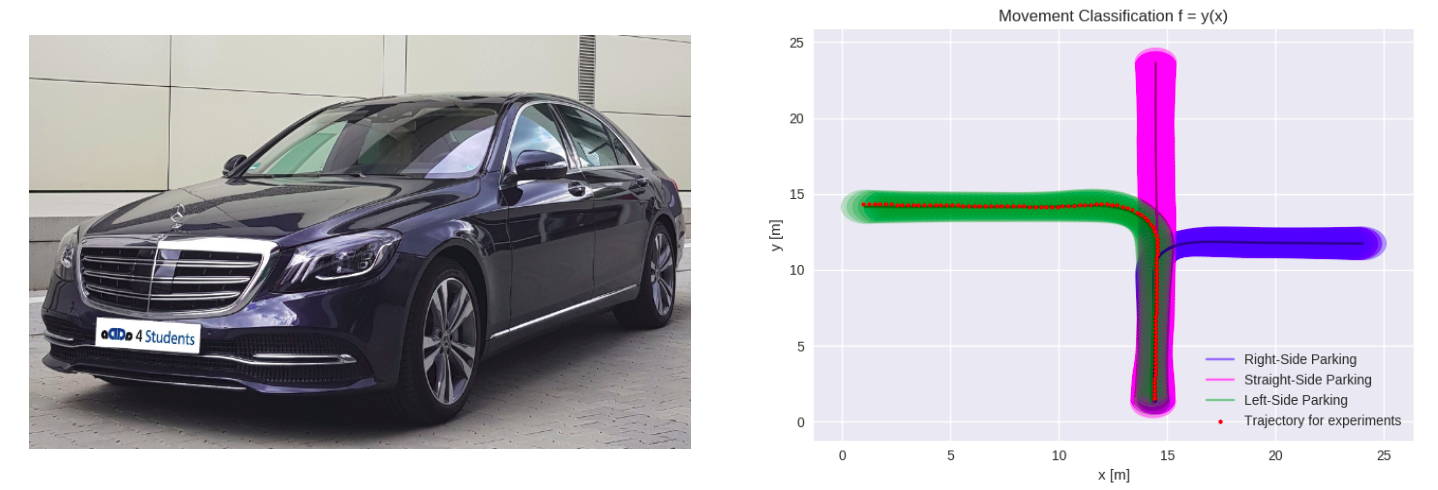
\includegraphics[width=14cm]{img/intro.png}
	\caption{The left side shows the \gls{aDDa} car, the right side illustrates the results of one of the experiments cases when the prediction, where the car is going, was made. Hereby the probabilistic model considers also the variance in the demonstrated trajectories, depicted in green, blue and pink}
	\label{fig:intro}    
\end{figure}

Even though to understand human behavior is a crucial task for further development of autonomous car, humans are very irrational and unpredictable and due to that, it is very hard to model them. However, in this document, we present a probabilistic intention prediction algorithm to predict motion and intentions from early observation for autonomous cars. To achieve this goal, the algorithm first learns the examples for all possible movement classes. When a car starts to move, it collects observations of the current position and predicts what intention for future movement is. Considering that the most important thing while driving is safety. We did a literature review which are the most common attacks on sensors (which information is using for prediction making) of autonomous car and made suggestions on how to protect the system from being attacked, as well as described the main privacy issues. \\
Probabilistic intention prediction algorithm was developed using two programming languages: Python and C++. The experiments were modeled and ran in \gls{ROS} environment. \gls{ROS} - an easy to use framework for developing robot software. In order to simplify the task for creating a complex robot model, it contains a lot of libraries and tools from a lot of robotic platforms. Additionally it has a wide community of users who provide big help while solving problems \cite{aboutROS}. \gls{RViz} was used as \gls{ROS} simulation visualization tool. \\
Beyond big giants like Tesla, Google, Aptiv, etc., chasing the dream of driverless cars, big number of academic institutions are also carrying out research in this field. \gls{TuD} has its own \gls{aDDa} working group \cite{aDDa}. \gls{aDDa} initiative started on February of $2017$. $8$ different departments at \gls{TuD} are working for one purpose to develop fully autonomous car by themselves, here, at University. All participants of the working group closely cooperate bringing together interdisciplinary know-how experience to jointly set up and operate an autonomous vehicle. One special feature of \gls{aDDa} is that the main work is done in the context of student projects (final thesis, semester work, permanent work at the team, etc.). By working together on the complex tasks of autonomous driving, participants are solving problems for tomorrow. \\
This thesis aims to investigate a probabilistic approach for intention prediction based in trajectory data. In particular, the approach is also tested with trajectory data, recorded with the real \gls{aDDa} car.

\section{Thesis Outline}

This thesis focuses on developing and evaluating probabilistic based movement and intention prediction algorithm. The thesis is organized as follows:

\begin{itemize}
	\item Chapter $2$. \textbf{Literature Review} focuses on the literature review on the intention prediction.
	\item Chapter $3$. \textbf{Probabilistic Trajectory Prediction} describes theoretical tools which help to formalize the problem for intention prediction.
	\item Chapter $4$. \textbf{Setup and Implementation} defines how and why simulation was set the way in was. Defines inputs for the system and experiments.	
	\item Chapter $5$. \textbf{Experiments and Results} describes experiments which were done during the thesis writing period and evaluate results which were received by performing various experiments.
	\item Chapter $6$. \textbf{Security Aspects} is based on the fact that "there is no safety without security" and tries to explain the main security and privacy issues of autonomous cars related to movement predictions.
	\item Chapter $7$. \textbf{Conclusion and Future Works} wind up this thesis with conclusions and future works based on the findings of previous chapters.
\end{itemize}